\apendice{Descripción de adquisición y tratamiento de datos}
\section{Descripción formal de los datos}

Como se ha especificado en la memoria, en el proyecto no se utilizan datos de fuentes externas, todos los datos son de elaboración propia.

Se pueden encontrar dos tipos de datos:
\begin{itemize}
    \item Proporcionados por el Usuario:
    \begin{itemize}
        \item Nombre del profesional. 
        \item Apellidos del profesional
        \item Contraseña para acceder al área.
        \item Nombre del paciente.
        \item Apellidos del paciente.
    \end{itemize}
        \item Datos recolectados por el dispositivo.
        \begin{itemize}
            \item Fecha y hora de cada medición.
            \item Los valores de fuerza/presión que ejerce cada dedo durante la medición:
            \begin{itemize}
                \item Pulgar en Kg
                \item Índice en Kg
                \item Corazón en Kg
                \item Anular en Kg
                \item Meñique en Kg
            \end{itemize}
        \end{itemize}
\end{itemize}

Los datos recogidos por el usuario tienen dos localizaciones finales. Aquellos relacionados con el profesional sanitario están recogidos en un archivo JSON, con una estructura interna tipo diccionario (clave: valor). Por otra parte, los datos de pacientes son almacenados en un archivo xlsx. Ambos archivos se encuentran cifrados para cumplir con la protección de datos.

Los datos recogidos por el sensor son números reales de hasta dos cifras decimales. Se almacenan en un archivo xlsx, donde se recogen los datos personales de los pacientes.
La unidad de medida es en Kilogramos (Kg), el rango de medida es desde 0 Kg hasta 4.5 Kg, con una frecuencia de parametrización de 0.5 Kg.

En la \textit{Figura} \ref{fig:Datosxlsx}, se puede observar el almacenamiento de los datos recogidos por el sensor. En cada hoja del xlsx se encuentran los datos recogidos, tanto de medición como nombre y apellidos de cada paciente. Además de los pesos, se recoge la fecha y hora de recogida de los datos. 
\begin{figure}
    \centering
    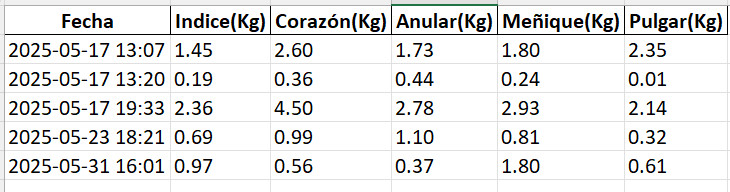
\includegraphics[width=0.8\linewidth]{img/Datos.png}
    \caption{Ejemplo de recogida de datos. Fuente propia}
    \label{fig:Datosxlsx}
\end{figure}
\section{Descripción clínica de los datos.}

El conjunto de datos corresponde a la cuantificación de la fuerza ejercida, con el fin de una evaluación terapéutica. Los valores registrados se estiman mediante una parametrización y el uso de la interpolación lineal de los valores obtenidos por los sensores.

La escala de medidas utilizada, de 0 Kg a 4.5Kg, se basa en el estudio 'Dispositivo de medición de fuerza de los dedos y su rol en el seguimiento de las funciones de la mano'  \cite{GOMEZ2022}. Los investigadores estudian la fuerza ejercida por cada dedo de veinte sujetos con edades comprendidas entre veinte y cuarenta años.

En la tabla \ref{tab:medidas_dedos}, se puede observar los resultados medios en el estudio. 

\begin{table}[h]
    \begin{tabular}{|l|l|l|l|l|l|}
\hline
\rowcolor[HTML]{BFBFBF} 
    Mano & Pulgar (N) & Índice (N) & Medio (N) & Anular (N)& Meñique (N) \\ \hline 
    Izquierda & 32.88 & 29.64 & 29.42 & 29.32 & 25.86 \\ \hline
    Derecha & 34.43 & 31.48 & 31.42 & 30.96 & 27.08 \\ \hline
    \end{tabular}
    \caption{Medidas de los dedos de ambas manos}
    \label{tab:medidas_dedos}
\end{table}

La recolección de los datos, permiten a los profesionales identificar diferentes patrones de evolución de los pacientes de manera individual, ya sean mejoras, pérdidas o estabilidad sin progreso de fuerza. Facilitando así, la personalización de los tratamientos o el cese de estos.